%\documentclass[
  bibliography=totoc,     % Literatur im Inhaltsverzeichnis
  captions=tableheading,  % Tabellenüberschriften
  titlepage=firstiscover, % Titelseite ist Deckblatt
]{scrartcl}

% Paket float verbessern
\usepackage{scrhack}

% Warnung, falls nochmal kompiliert werden muss
\usepackage[aux]{rerunfilecheck}

% unverzichtbare Mathe-Befehle
\usepackage{amsmath}
% viele Mathe-Symbole
\usepackage{amssymb}
% Erweiterungen für amsmath
\usepackage{mathtools}

% Fonteinstellungen
\usepackage{fontspec}
% Latin Modern Fonts werden automatisch geladen
% Alternativ zum Beispiel:
%\setromanfont{Libertinus Serif}
%\setsansfont{Libertinus Sans}
%\setmonofont{Libertinus Mono}

% Wenn man andere Schriftarten gesetzt hat,
% sollte man das Seiten-Layout neu berechnen lassen
\recalctypearea{}

% deutsche Spracheinstellungen
\usepackage[ngerman]{babel}


\usepackage[
  math-style=ISO,    % ┐
  bold-style=ISO,    % │
  sans-style=italic, % │ ISO-Standard folgen
  nabla=upright,     % │
  partial=upright,   % │
  mathrm=sym,        % ┘
  warnings-off={           % ┐
    mathtools-colon,       % │ unnötige Warnungen ausschalten
    mathtools-overbracket, % │
  },                       % ┘
]{unicode-math}

% traditionelle Fonts für Mathematik
\setmathfont{Latin Modern Math}
% Alternativ zum Beispiel:
%\setmathfont{Libertinus Math}

\setmathfont{XITS Math}[range={scr, bfscr}]
\setmathfont{XITS Math}[range={cal, bfcal}, StylisticSet=1]

% Zahlen und Einheiten
\usepackage[
  locale=DE,                   % deutsche Einstellungen
  separate-uncertainty=true,   % immer Unsicherheit mit \pm
  per-mode=symbol-or-fraction, % / in inline math, fraction in display math
]{siunitx}

% chemische Formeln
\usepackage[
  version=4,
  math-greek=default, % ┐ mit unicode-math zusammenarbeiten
  text-greek=default, % ┘
]{mhchem}

% richtige Anführungszeichen
\usepackage[autostyle]{csquotes}

% schöne Brüche im Text
\usepackage{xfrac}

% Standardplatzierung für Floats einstellen
\usepackage{float}
\floatplacement{figure}{htbp}
\floatplacement{table}{htbp}

% Floats innerhalb einer Section halten
\usepackage[
  section, % Floats innerhalb der Section halten
  below,   % unterhalb der Section aber auf der selben Seite ist ok
]{placeins}

% Seite drehen für breite Tabellen: landscape Umgebung
\usepackage{pdflscape}

% Captions schöner machen.
\usepackage[
  labelfont=bf,        % Tabelle x: Abbildung y: ist jetzt fett
  font=small,          % Schrift etwas kleiner als Dokument
  width=0.9\textwidth, % maximale Breite einer Caption schmaler
]{caption}
% subfigure, subtable, subref
\usepackage{subcaption}

% Grafiken können eingebunden werden
\usepackage{graphicx}

% schöne Tabellen
\usepackage{tabularray}
\UseTblrLibrary{booktabs, siunitx}

% Verbesserungen am Schriftbild
\usepackage{microtype}

% Literaturverzeichnis
\usepackage[
  backend=biber,
]{biblatex}
% Quellendatenbank
\addbibresource{lit.bib}
\addbibresource{programme.bib}

% Hyperlinks im Dokument
\usepackage[
  german,
  unicode,        % Unicode in PDF-Attributen erlauben
  pdfusetitle,    % Titel, Autoren und Datum als PDF-Attribute
  pdfcreator={},  % ┐ PDF-Attribute säubern
  pdfproducer={}, % ┘
]{hyperref}
% erweiterte Bookmarks im PDF
\usepackage{bookmark}

% Trennung von Wörtern mit Strichen
\usepackage[shortcuts]{extdash}

\author{%
  Vincent Wirsdörfer\\%
  \href{mailto:vincent.wirsdoerfer@udo.edu}{authorA@udo.edu}%
  \and%
  Joris Daus\\%
  \href{mailto:joris.daus@udo.edu}{authorB@udo.edu}%
}
\publishers{TU Dortmund – Fakultät Physik}


%\begin{document}
\section{Diskussion}
\label{sec:Diskussion}

Insgesamt sind die Ergebnisse des Versuches als positiv zu bewerten. In den meisten Fällen zeigt der Abgleich der 
Werte für die jeweiligen Leitfähigkeitsparameter mit der Literatur keine signifikante Abweichung der Größenordnung.
Unglücklicherweise sind in der Versuchsanleitung keine Vergleichswerte angegeben und aufgrund der Spezifität der 
untersuchten mikroskopischen Größen, sind häufig keine Literaturwerte zu finden.\\

\noindent Nichtsdestotrotz kann gesagt werden, dass sich alle Ladungsträgerdichten in einer vertrauenswürdigen Größenordnung befinden:

\begin{align*}
    n_\text{Silber} = \left(1.18 \pm 0.20\right)\cdot{}10^{29}\,\unit{\per\cubic\meter}\\
    n_\text{Kupfer} = \left(1.29 \pm 0.22\right)\cdot{}10^{29}\,\unit{\per\cubic\meter}\\
    n_\text{Zink}   = \left(8.90 \pm 1.30\right)\cdot{}10^{28}\,\unit{\per\cubic\meter}\\
\end{align*}

\noindent Diese Werte beziehen sich jedoch ausschließlich auf die Messung der Hall-Spannung mittels wechselndem B-Feld.
Für die Messung bei konstantem Magnetfeld beträgt der gemessene Wert der Ladungsträgerdichte für Silber 
$n_\text{Silber} = \left(6.80 \pm 1.10\right)\cdot{}10^{27}\,\unit[per-mode=reciprocal]{\per\cubic\meter}$. Ein zum Vergleich naheliegender
Literaturwert ist die Ladungsträgerdichte von Kupfer mit $n_\text{Kupfer,Lit} = 8.4\cdot{}10^{28}\,\unit[per-mode=reciprocal]{
\per\cubic\meter}$\cite{leitfaehigkeiten}.\\

\noindent Auch die gemessenen Werte der Driftgeschwindigkeit aller Metalle mit 

\begin{align*}
    v_\text{d,Silber} = \left(5.3 \pm 0.9\right)\cdot{}10^{-5}\,\unit{\meter\per\second}\\
    v_\text{d,Kupfer} = \left(4.8 \pm 0.8\right)\cdot{}10^{-5}\,\unit{\meter\per\second}\\
    v_\text{d,Zink}   = \left(7.0 \pm 1.0\right)\cdot{}10^{-5}\,\unit{\meter\per\second}\\
\end{align*}

\noindent zeigen in der Größenordnung eine reliable Zuverlässigkeit, das beispielsweise der Literaturwert von Kupfer bei 
$v_\text{Lit} = 9.8\cdot{}10^{-5}\unit[per-mode=reciprocal]{\meter\per\second}$ liegt.\\

\noindent Gleiches gilt für den Proportionalitätsfaktor zwischen Driftgeschwindigkeit und elektrischem Feld, der 
sogenannten Beweglichkeit $\mu$. Hier lauten die gemessenen Werte 

\begin{align*}
    \mu_\text{Silber} &= \left(2.70 \pm0.50\right)\cdot{}10^{-3}\,\unit{\square\meter\per\volt\per\second}\\
    \mu_\text{Kupfer} &= \left(3.10 \pm0.50\right)\cdot{}10^{-3}\,\unit{\square\meter\per\volt\per\second}\\
    \mu_\text{Zink  } &= \left(1.20\pm 0.20\right)\cdot{}10^{-3}\,\unit{\square\meter\per\volt\per\second}.\\
\end{align*}

\noindent Der Literaturwert von Kupfer \cite[292]{Physikalisches_Praktikum} liegt bei diesem Parameter bei $\mu_\text{Kupfer,Lit} = 3.2
\cdot{}10^{-3}\,\unit[per-mode=reciprocal]{\square\meter\per\volt\per\second}$, sodass der gemessene Wert mit Fehlertoleranz dem tatsächlichen 
Wert gleicht.\\

\noindent Für die mittlere Flugzeit wurden folgende Werte aufgenommen:

\begin{align*}
    \bar{\tau}_\text{Silber} = \left(3.10\pm0.50\right)\cdot10^{-14}\,\unit{\second}\\
    \bar{\tau}_\text{Kupfer} = \left(3.50\pm0.60\right)\cdot10^{-14}\,\unit{\second}\\
    \bar{\tau}_\text{Zink} =   \left(1.35\pm0.19\right)\cdot10^{-14}\,\unit{\second}.\\
\end{align*}

\noindent Hierbei sind jedoch keine zuverlässigen Quellen auffindbar, weshalb der direkte Abgleich schwierig ist. 
Dessen ungeachtet ist nach Gleichung \eqref{eqn:Beweglichkeit} die mittlere Flugzeit nur um einen Vorfaktor von der 
Beweglichkeit verschieden. Die guten Ergebnisse der Beweglichkeit werden wohl somit höchstwahrscheinlich auch auf die 
mittlere Flugzeit übertragbar sein. Ähnliches gilt für die Totalgeschwindigkeit der Elektronen in den Leitern und für 
die mittlere freie Weglänge. Hierfür sind ebenfalls keine Vergleichswerte vorhanden, jedoch ist die Ladungsträgerdichte 
ausschlaggebend für die Fermie-Energie, welche nach der Fermi-Dirac-Verteilung die Totalgeschwindigkeit bestimmt. Somit 
besteht die Vermutung, dass die zuverlässigen Parameter durch mathematische Verknüpfungen auch einen positiven Einfluss 
auf die anderen Größen haben, obwohl der dabei entstehende Fehler nach der \emph{Gauß'schen Fehlerfortpflanzung} 
selbstverständlich wächst.\\ 
\noindent Anhand des Vorfaktors von Gleichung \eqref{eqn:Spannung} kann determiniert werden, ob es sich bei der Probe um 
einen Löcherleiter oder um einen Elektronenleiter handelt. Da in allen Fällen positive Steigungen zu sehen sind, kann gefolgert 
werden, dass Kupfer, Silber und Zink Elektronenleiter sind. Vergleicht man dies mit der Literatur, so ist das Ergebnis für 
Kupfer und Silber richtig, jedoch nicht für Zink \cite{Elektronenleiter}. Dies kann an einem systematischen Fehler liegen, 
dass die Polung nicht richtig ist. Das bedeutet, dass Zink unwissenhaft eine inverse Polung verwendet wurde.
Der Vollständigkeit halber nun noch die Werte der Totalgeschwindigkeit

\begin{align*}
    v_\text{Silber} = \left(1.76\pm0.10\right)\cdot10^{6}\,\unit{\meter\per\second}\\
    v_\text{Kupfer} = \left(1.81\pm0.10\right)\cdot10^{6}\,\unit{\meter\per\second}\\
    v_\text{Zink}   = \left(1.60\pm0.08\right)\cdot10^{6}\,\unit{\meter\per\second}\\
\end{align*}

\noindent und der mittleren freien Weglänge

\begin{align*}
    \bar{l}_\text{Silber} &= \left(5.50\pm0.60\right)\cdot10^{-8}\,\unit{\meter}\\
    \bar{l}_\text{Kupfer} &= \left(6.30\pm0.70\right)\cdot10^{-8}\,\unit{\meter}\\
    \bar{l}_\text{Kupfer} &= \left(2.16\pm0.21\right)\cdot10^{-8}\,\unit{\meter}.\\
\end{align*}

\noindent Wie bereits in der Einleitung der Diskussion angeklungen, besteht das größte Problem darin, seriöse 
Quellen für vergleichbare Literaturwerte zu finden. Diese Problematik erschwert die Interpretation bzw. Bewertung 
der Ergebnisse signifikant. Nichtsdestotrotz können vereinzelnd Vergleichswerte für bestimmte Größen gefunden werden, 
welche über mathematische Korrelationen grobe Aussagen über die Richtigkeit weiterer Parameter erlauben. Ferner 
könnten die folgenden systematischen Fehler, welche bei der Versuchsdurchführung beobachtet werden, Grund für 
Abweichungen der Messwerte sein:\\

\noindent Die zu messende Hall-Spannung befindet sich stetig in einem niedrigen $\unit{\milli\volt}$ Bereich und ist 
aufgrund der Versuchskonstruktion extrem empfindlich und anfällig für Änderungen. So springt der Wert beim Ablesen am 
digitalen Spannungsmessgerät oftmals zwischen zwei Werten, was die korrekte Notation erschwert. Eine vergleichbare Komplikation 
ergibt sich bei der Messung des magnetischen Feldes mit der Hall-Sonde. Auch hier springt der Wert der Feldstärke 
aufgrund von Inhomogenitäten zwischen den Polschuhen und Erhitzung der Spulen. Der soeben genannte thermische Aspekt 
der Spulen hat bei der Versuchsreihe mit konstantem B-Feld eine noch markantere Auswirkung. Wegen Erhitzung entstehen 
Verluste, weshalb der tatsächliche Wert des Magnetfeldes bei den verschiedenen Querströmen vermutlich auch variiert.
Dies könnte beispielsweise ein Grund für die Abweichung der Ladungsträgerdichte bei Silber sein.  

\section{Anhang}

\begin{figure}[H]
    \centering
    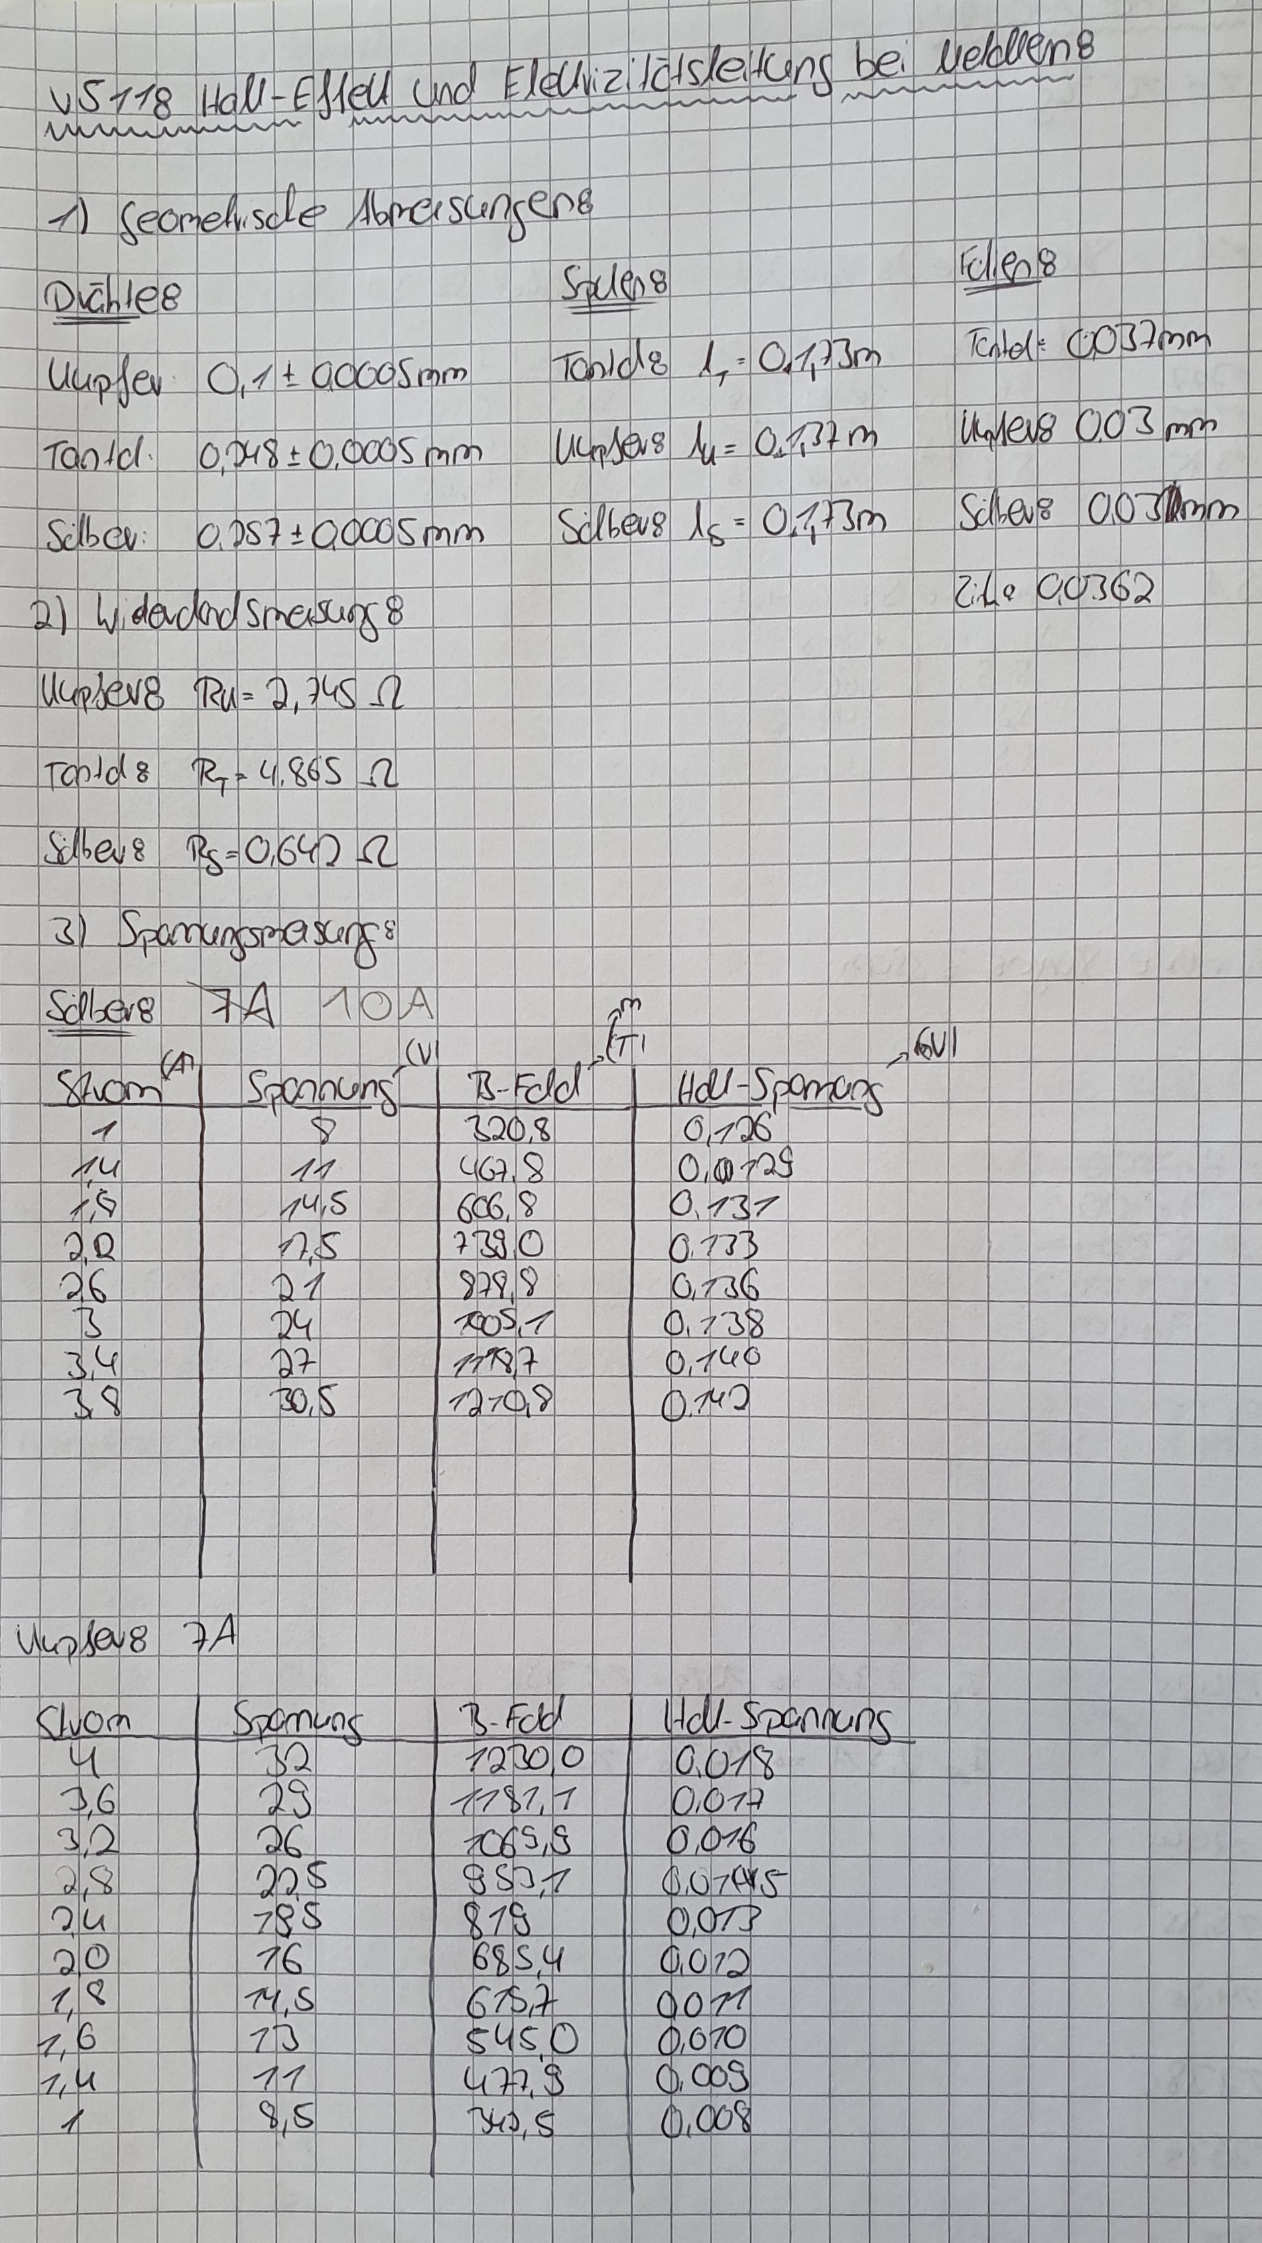
\includegraphics[width=\textwidth]{content/v511_Laborbuch1.jpg}
\end{figure}


\begin{figure}[H]
    \centering
    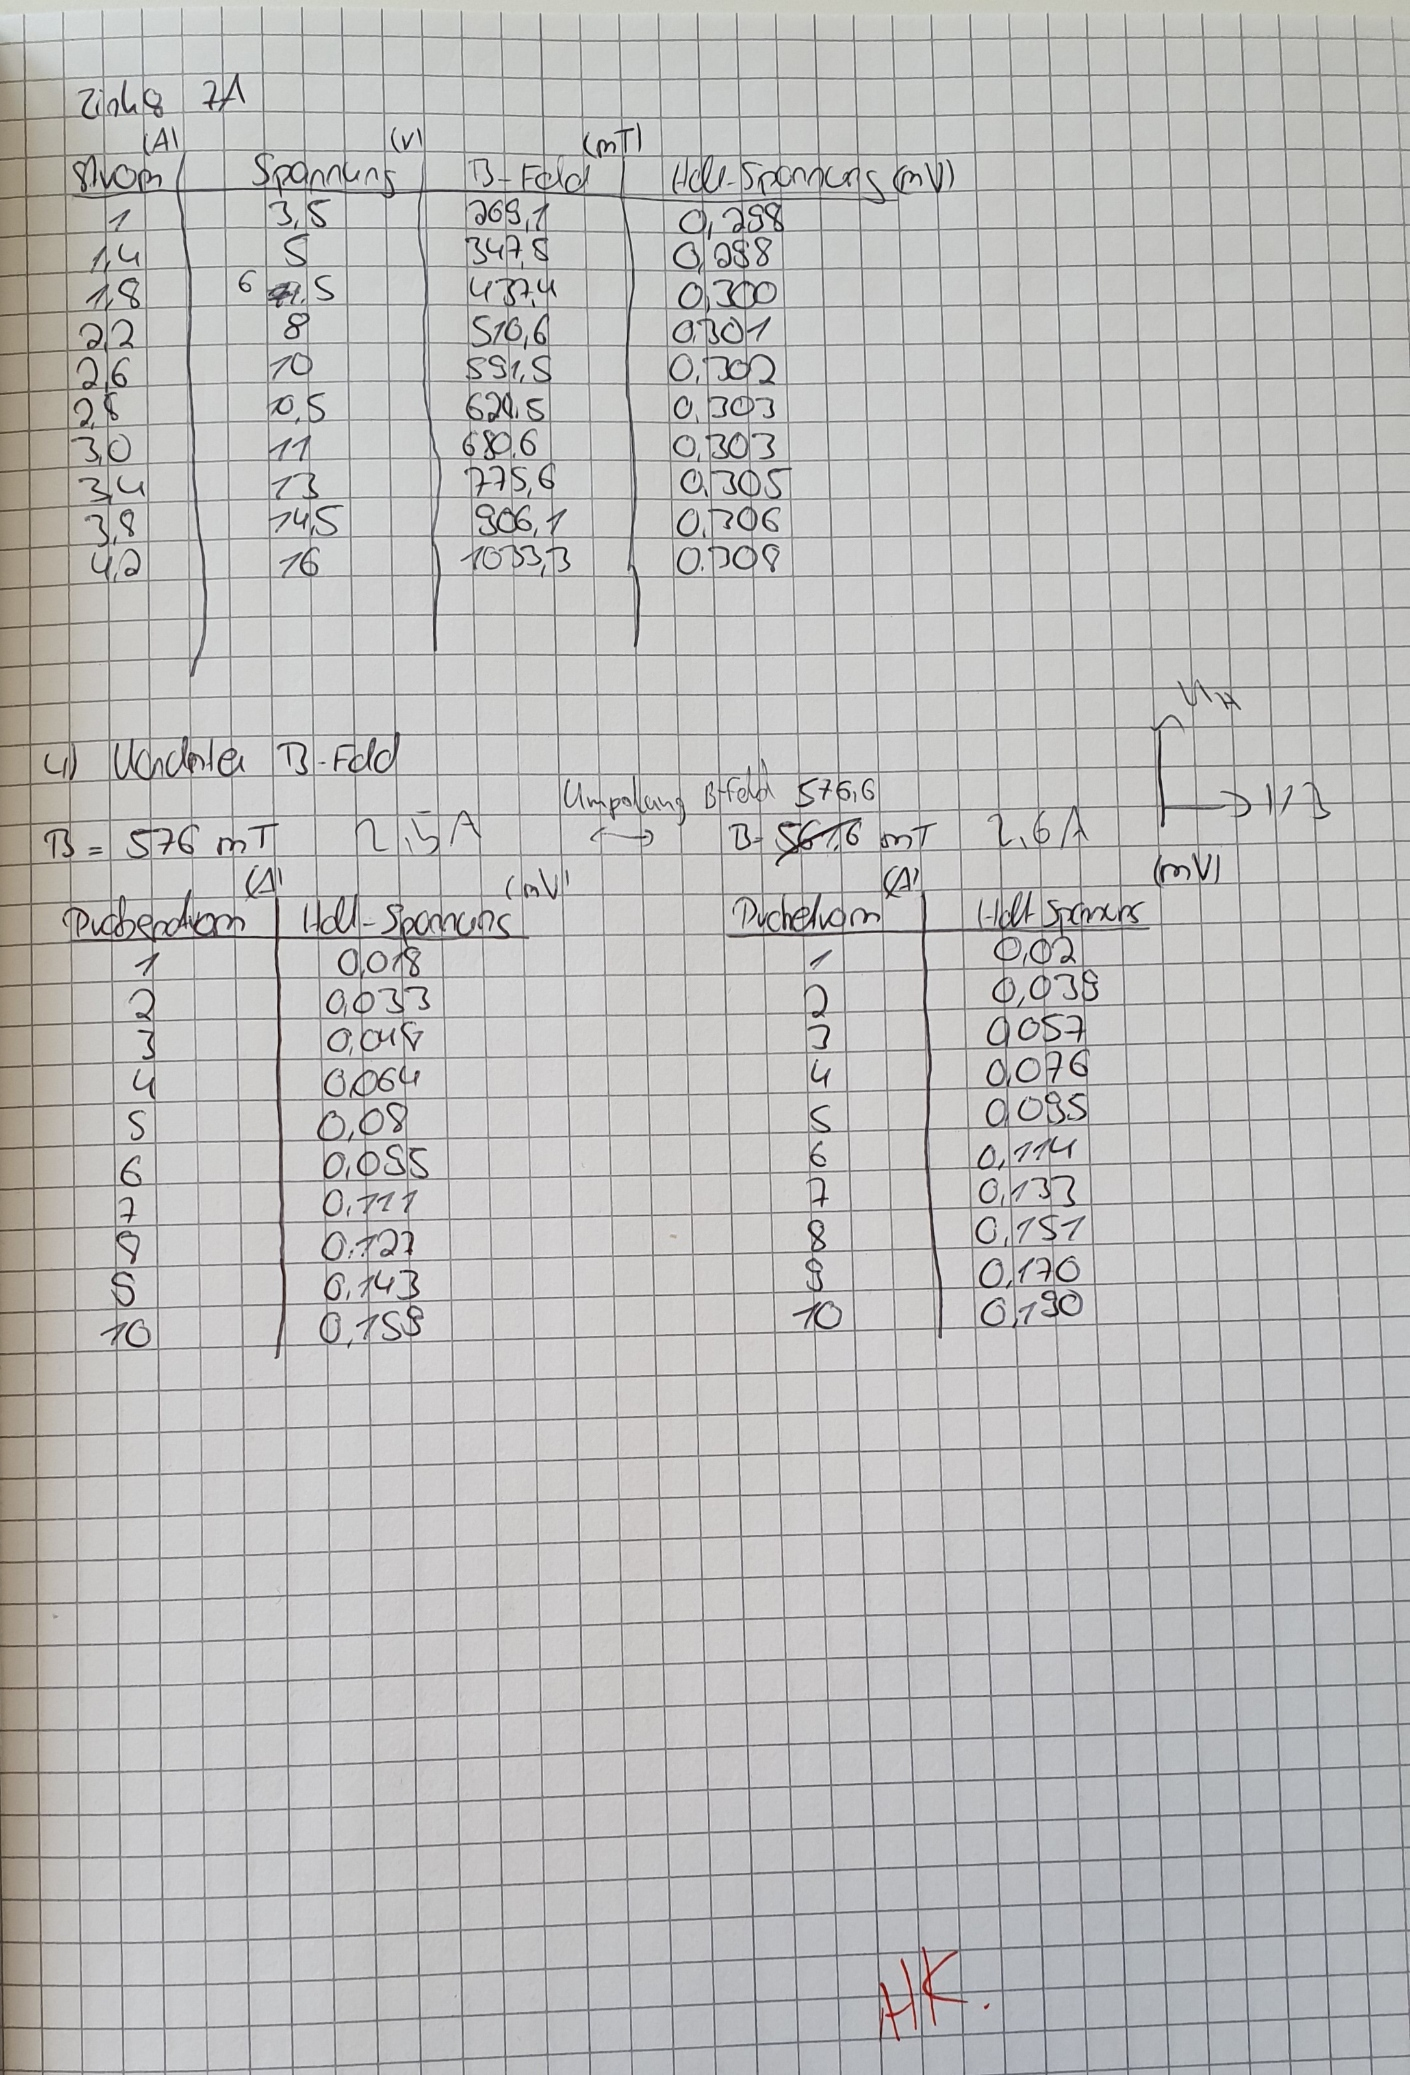
\includegraphics[width=\textwidth]{content/v511_Laborbuch2.jpg}
\end{figure}

%\end{document}









%Messmethode konstanter Probenstrom und B-Feld geändert: nur Aufladen bzw nur Entladung des Magneten, hätten eigentlich beides machen müssen
%Literaturwert Ladungsträgerdichte Kupfer: 8,4*10^28 https://13db.de/wissen/geschwindigkeit-von-elektronen/
%\cite{leitfaehigkeiten}
%wir haben: konstanten B-Feld:  (1.06+/-0.18)e+28 1/m^3 | konstanten Probenstrom:  (1.29+/-0.22)e+29 1/m^3 
%Extrapolation der linearen Regression geht bei nicht auf 0 für 0T (plot 1-3)
%hat auch zur Folge: nur positive Hallspannungen, daher keine Rückschlüsse auf positive oder negative Ladungsträger bzw Lücken
%Literaturwert: Quelle Geschke physikalischen Praktikum(schon in lit.bib) Seite 292 µ für Kupfer ist 32cm^2/(Vs) umgerechnet 3,2 10^-3 m^2/(Vs) wir haben 3.1+-0,5m^2/(Vs)!!!!!!
%\cite[292]{Physikalisches_Praktikum}
%sehr super sexy dass das das selbe ist njom njom
%Literaturwert Driftgeschwindigkeit in Kupfer 9,8e-5m/s https://13db.de/wissen/geschwindigkeit-von-elektronen/
%\cite{leitfaehigkeiten}
%wir haben 4,8+-0,8e-5m/s
%Messfehler: extrem kleine Spannungen, weshalb sehr empfindlich. außerdem hat die angezeigte Spannung sich durch bloßes berühren geändert, auch kein stabiler Wert angezeigt
%probenhalterung wackelig und daher wsl nt ganz orthogonal auf B-Feld
%Magnetspulen sind heiß geworden und daher verluste entstanden -> Magnetfeld wurde schwächer (vor allem bei Messung mit konstanten B-Feld wichtig)

